\documentclass[Rapport/Rapport_main.tex]{subfiles}
\begin{document}
\subsection{Cup holder}
Til at lave blokken Cup Holder, kombineres de to blokke Cup Light og Cup Sensor. For detaljeret forklaring refereres der til \fullref{hwdesign:sec:cupholder_hw_design} i Hardwaredesign bilaget.
\subsubsection{Hardwaredesign}
Der er designet printpladen som ses på figur \ref{fig:CupHolderPrintpladeDesign}. 

\begin{figure}[H]
\centering
\makebox[\textwidth][c]{%
\begin{subfigure}{.55\textwidth}
  \centering
        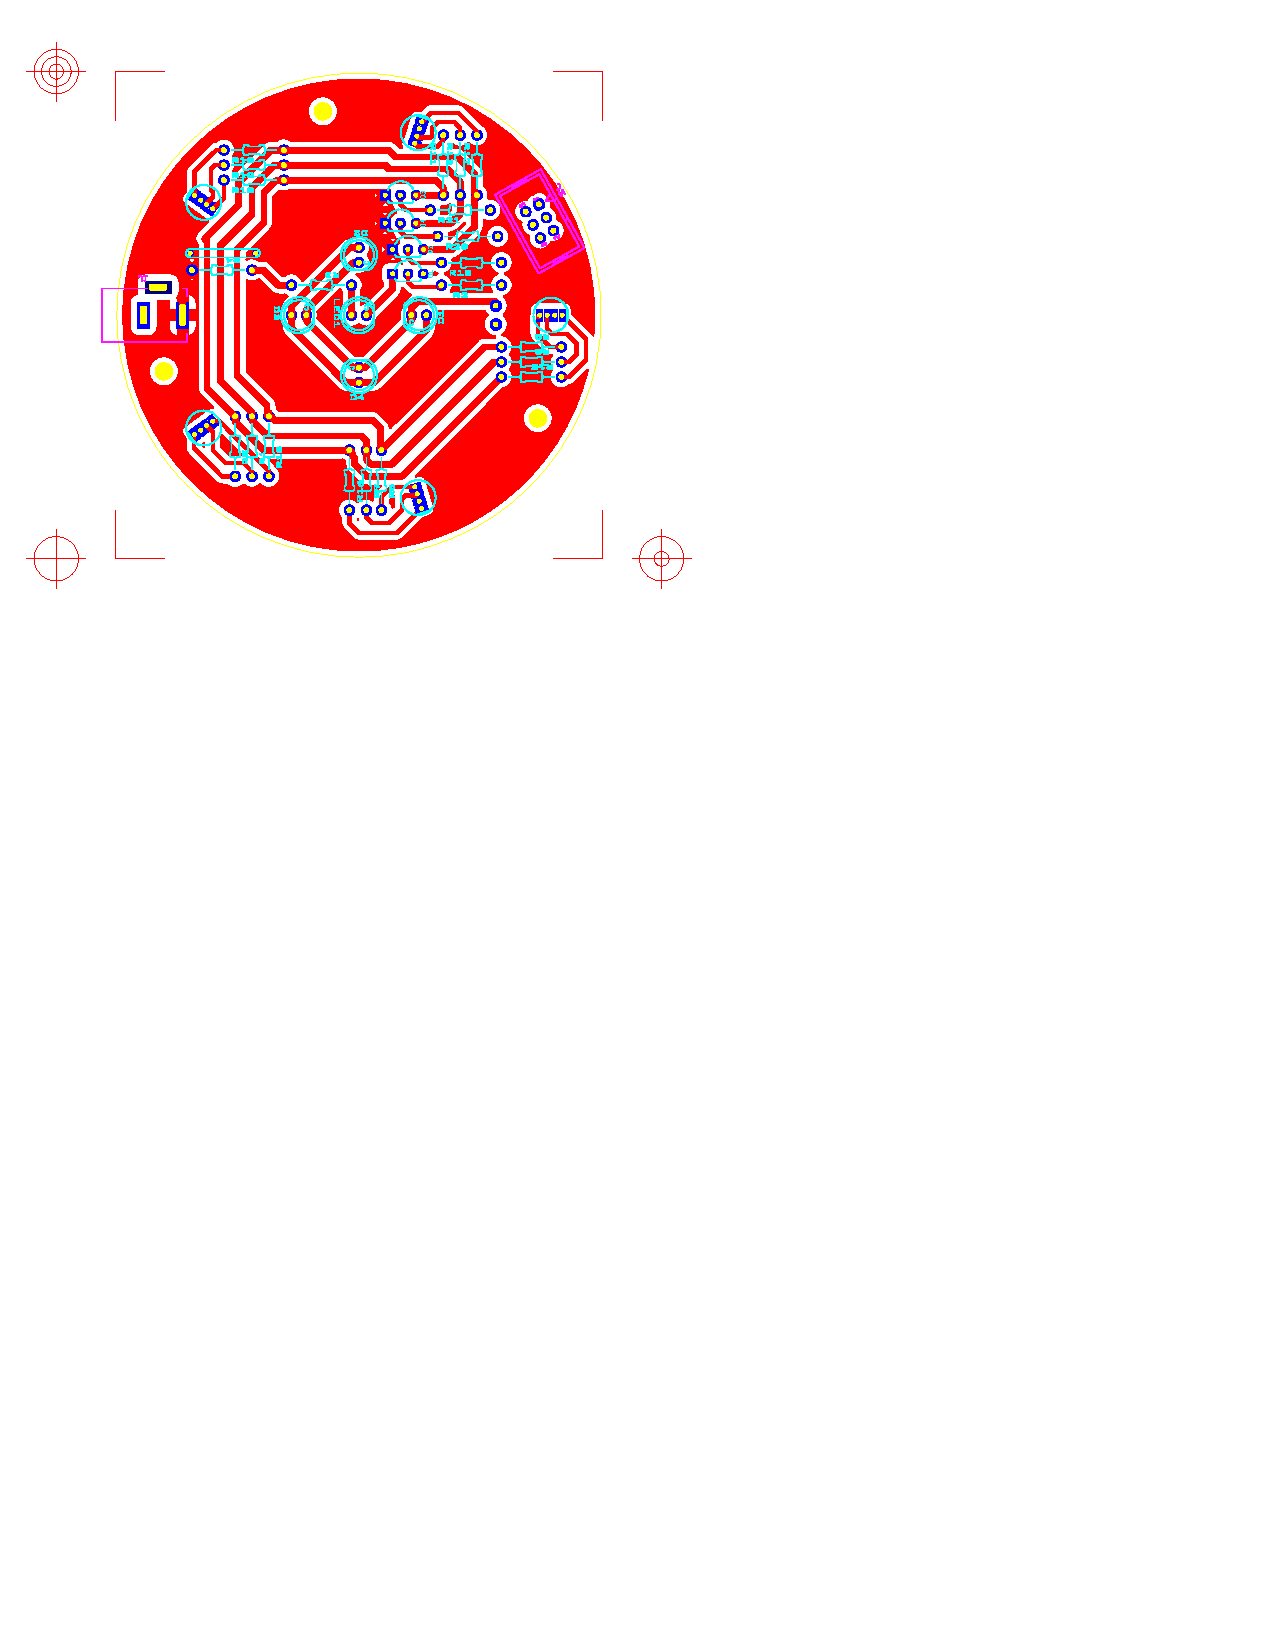
\includegraphics[width=1\linewidth,trim={0.6in 7.28in 4.5in 0.5in},clip, page=1]{HardwareDesign/CupHolder/graphics/bund.pdf}
\end{subfigure}%
\begin{subfigure}{.55\textwidth}
  \centering
    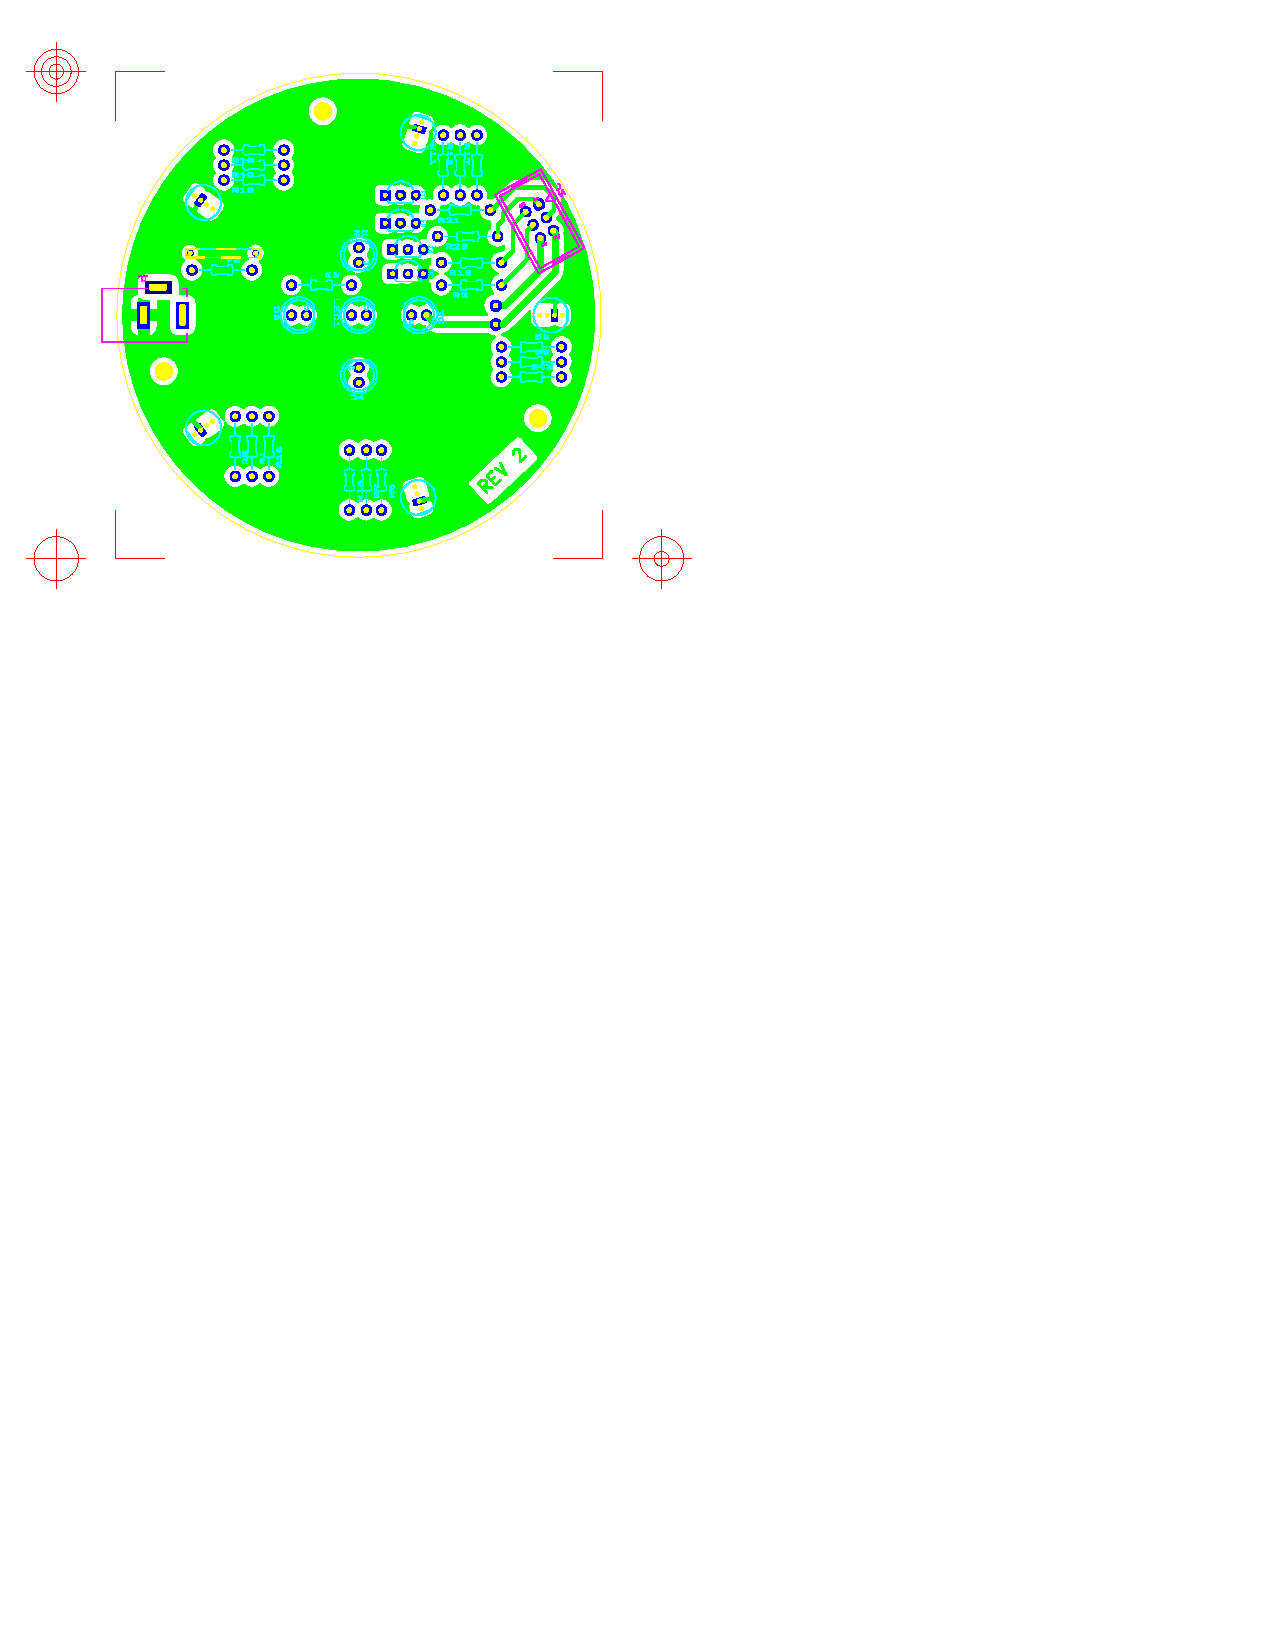
\includegraphics[width=1\linewidth,trim={0.6in 7.28in 4.5in 0.5in},clip, page=1]{HardwareDesign/CupHolder/graphics/top.pdf}
\end{subfigure}
}
\caption{Design af printplade. På venstre figur er det røde areal kobberet på undersiden af printpladen, og på højre figur er det grønne areal kobberet på oversiden. Den cyane farve er silkscreen på toppen, som viser hvilke komponenter, der er på oversiden. Den lilla farve er silkscreen på bunden og indikerer komponenter der sidder på bunden}
\label{fig:CupHolderPrintpladeDesign}
\end{figure}

Som en del af designet af printpladen er der fokus på minimering af støj, men også på de fysiske dimensioner. Komponenterne placeres i forhold til kravene fra Cup Sensor (figur \ref{fig:lightPaht}) og fra (kravspecifikationen (K\ref{kravspec:req:light-D-center} og K\ref{kravspec:req:light-led-angle} i kravspecifikation bilaget).

\subsubsection{Implementering}
Resultatet af printpladen kan ses på figur \ref{fig:CupHolderRev2}.
\begin{figure}[H]
\centering
\makebox[\textwidth][c]{%
\begin{subfigure}{.53\textwidth}
  \centering
        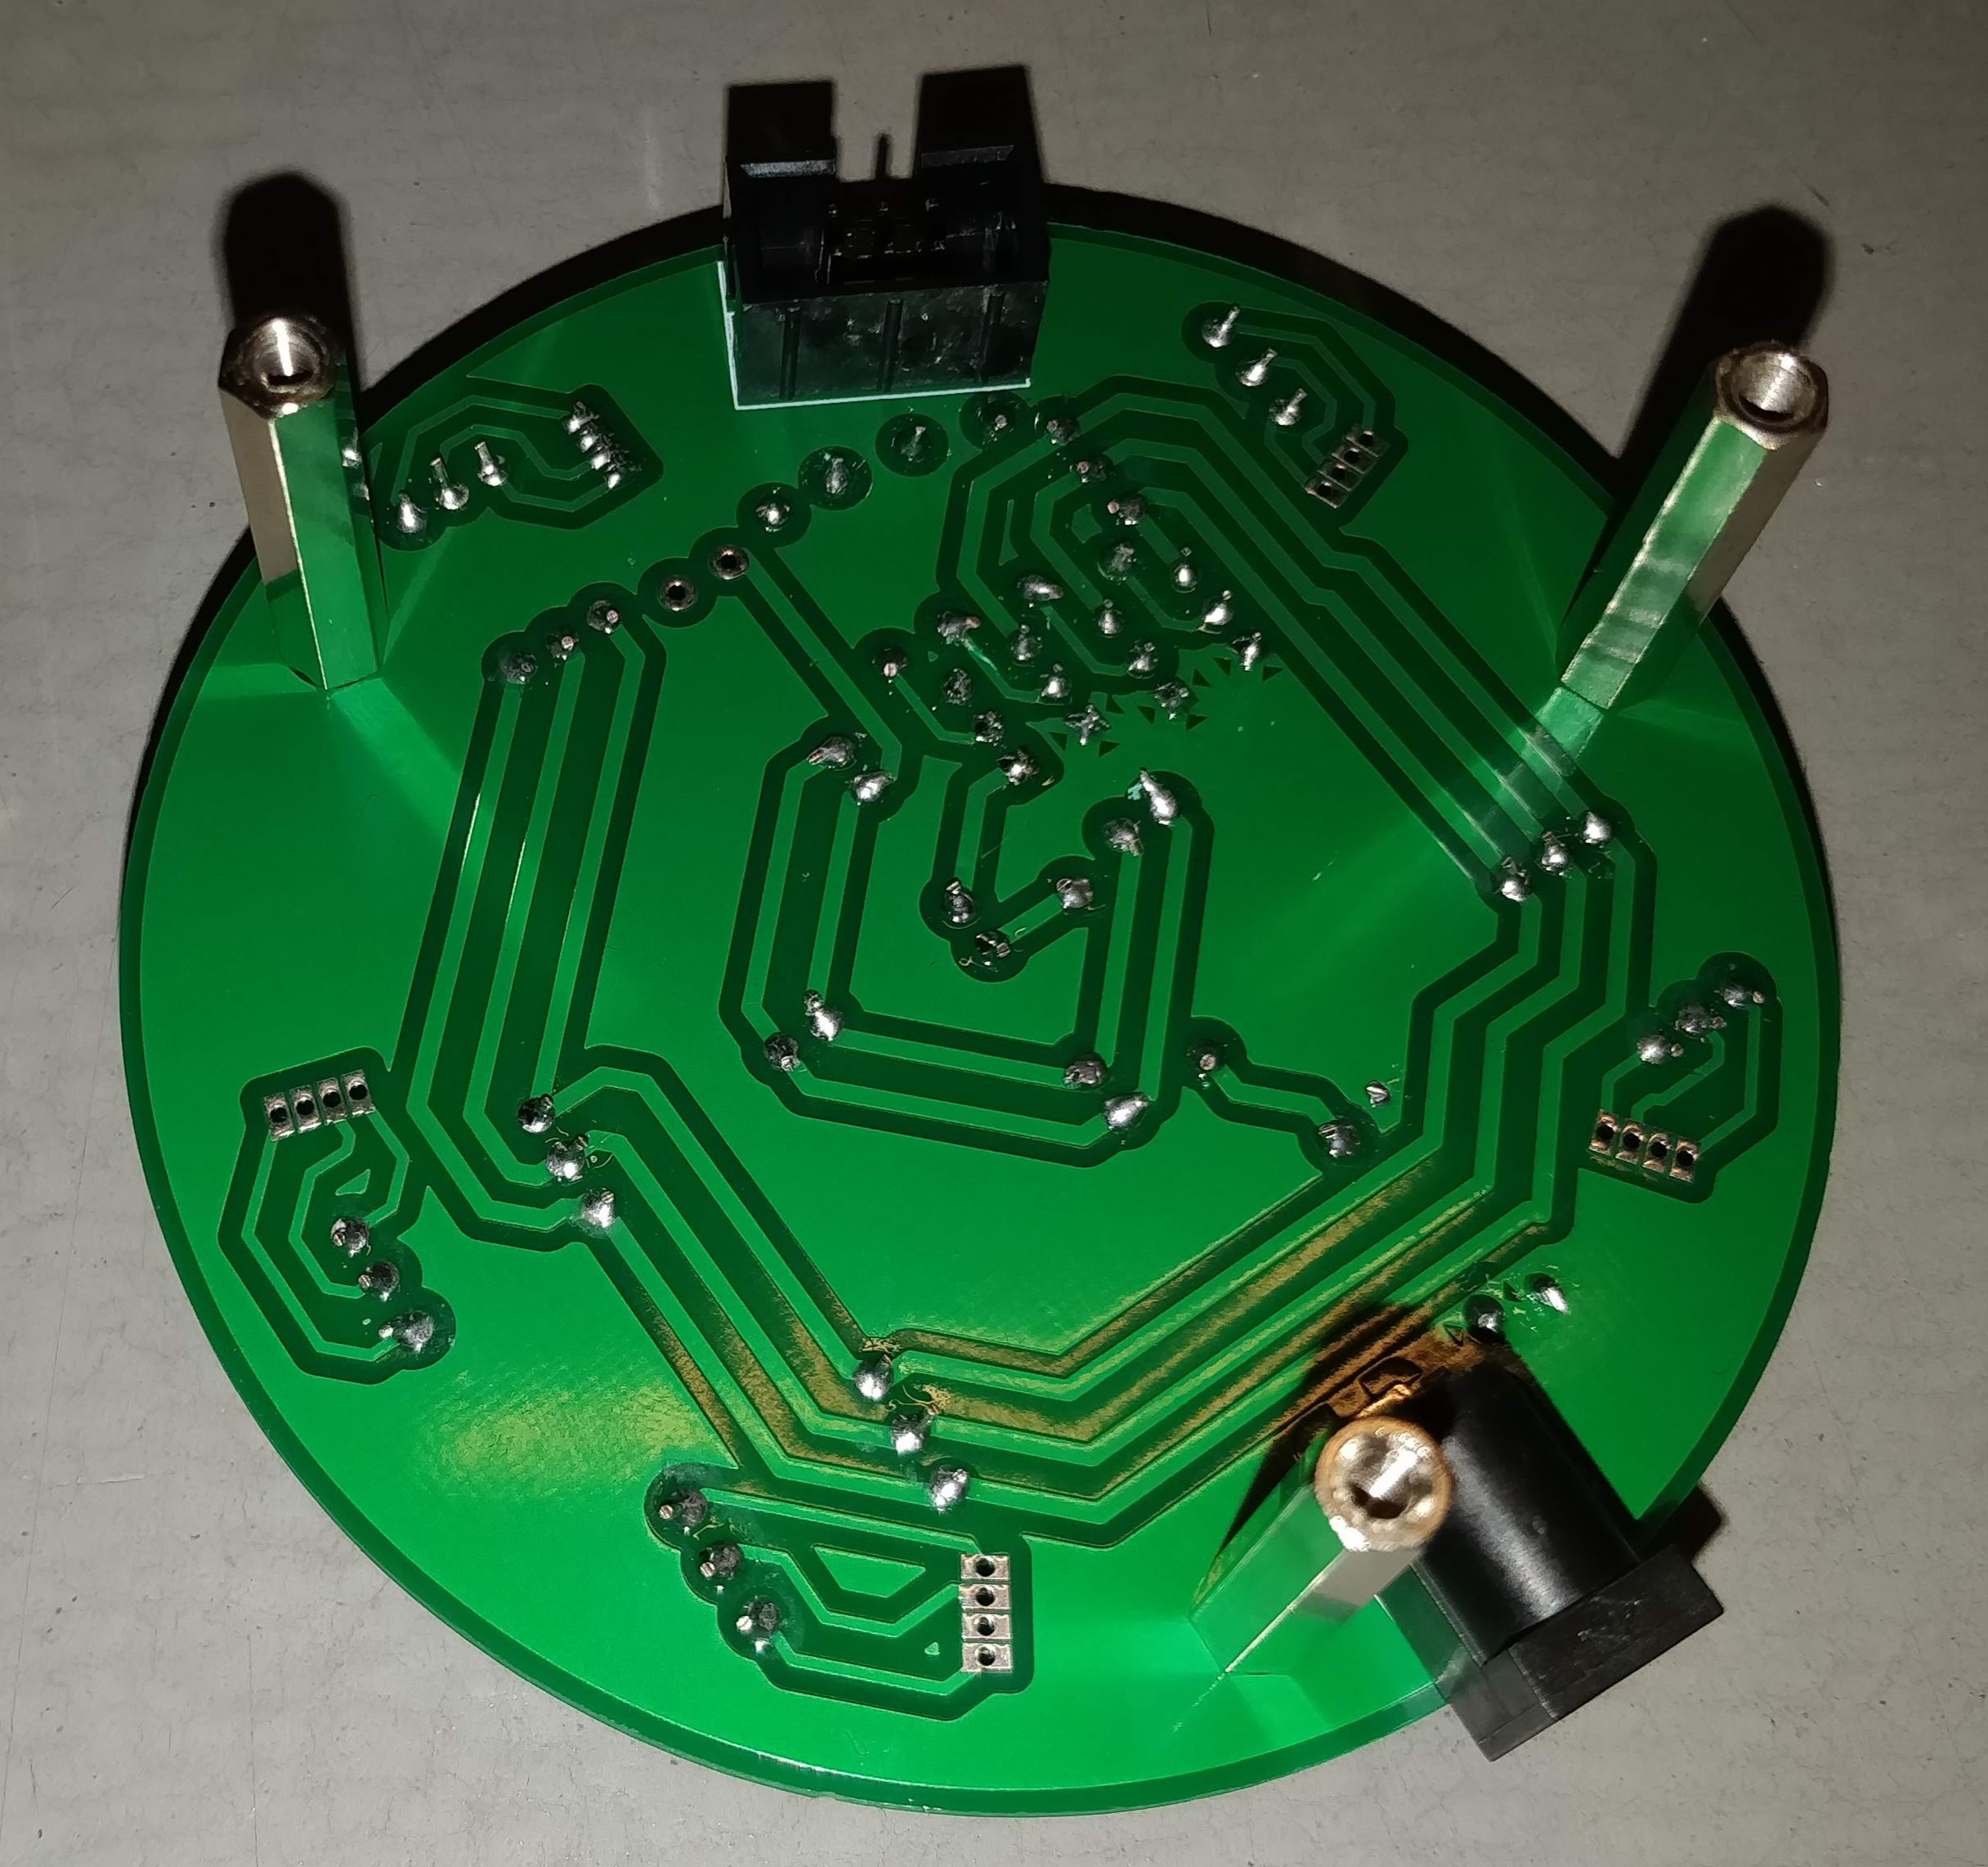
\includegraphics[width=1\linewidth]{HardwareDesign/CupHolder/graphics/bund_rev_2.jpg}
\end{subfigure}%
\begin{subfigure}{.57\textwidth}
  \centering
    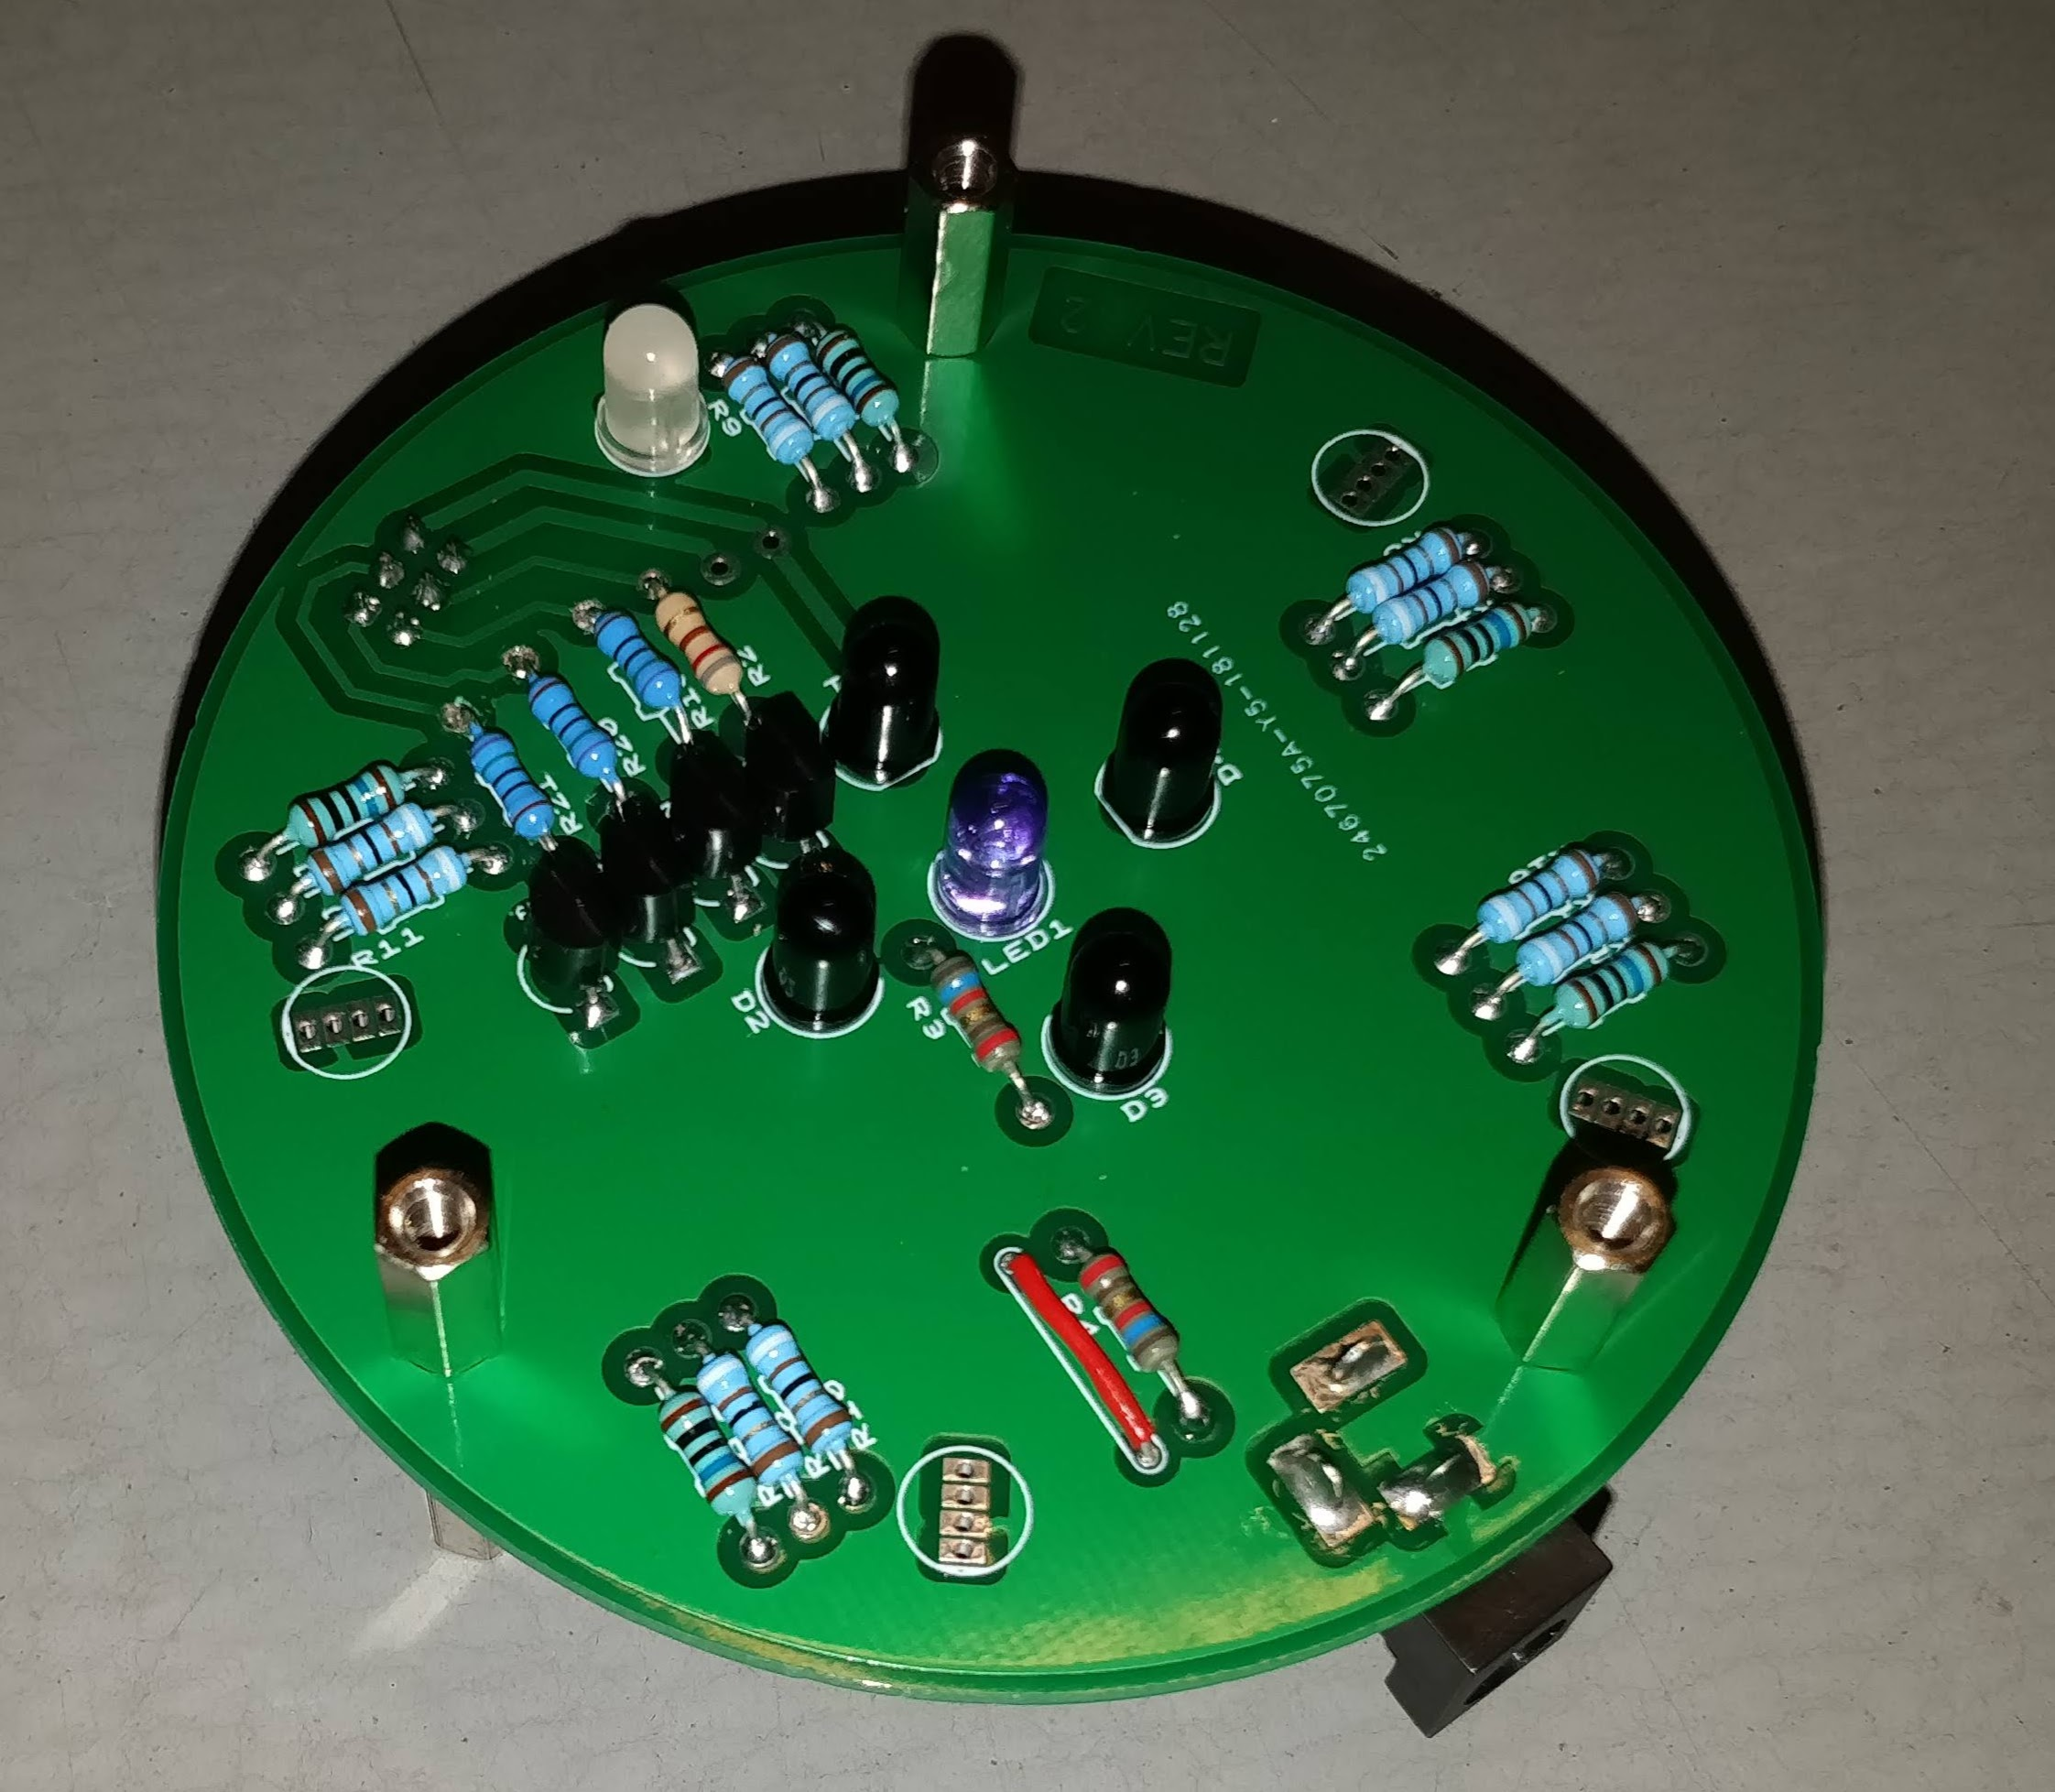
\includegraphics[width=1\linewidth]{HardwareDesign/CupHolder/graphics/top_rev_2.jpg}
\end{subfigure}
}
\caption{Den anden version af Cup Holder printplade (REV 2), som blev produceret i Kina, hvor der er gennemplatering, soldermaske og silkscreen. På venstre figur ses bunden af printpladen. På højre side figur ses toppen af printpladen.}
\label{fig:CupHolderRev2}
\end{figure}

\end{document}